\documentclass[twocolumn,a4j]{jsarticle}
\setlength{\topmargin}{-20.4cm}
\setlength{\oddsidemargin}{-10.4mm}
\setlength{\evensidemargin}{-10.4mm}
\setlength{\textwidth}{18cm}
\setlength{\textheight}{26cm}

\usepackage[top=15truemm,bottom=25truemm,left=15truemm,right=15truemm]{geometry}
\usepackage[latin1]{inputenc}
\usepackage{amsmath}
\usepackage{amsfonts}
\usepackage{amssymb}
\usepackage[dvipdfmx]{graphicx}
\usepackage[dvipdfmx]{color}
\usepackage{listings}
\usepackage{listings,jvlisting}
\usepackage{geometry}
\usepackage{framed}
\usepackage{color}
\usepackage[dvipdfmx]{hyperref}
\usepackage{ascmac}
\usepackage{enumerate}
\usepackage{tabularx}
\usepackage{cancel}
\usepackage{scalefnt}

\renewcommand{\figurename}{Fig.}
\renewcommand{\tablename}{Table }

\lstset{
basicstyle={\ttfamily},
identifierstyle={\small},
commentstyle={\smallitshape},
keywordstyle={\small\bfseries},
ndkeywordstyle={\small},
stringstyle={\small\ttfamily},
frame={tb},
breaklines=true,
columns=[l]{fullflexible},
xrightmargin=0zw,
xleftmargin=3zw,
numberstyle={\scriptsize},
stepnumber=1,
numbersep=1zw,
lineskip=-0.5ex
}

\makeatletter
\def\@maketitle
{
\begin{center}
{\LARGE \@title \par}
\end{center}
\begin{flushright}
{\large 報告書 NO.07 - 2\quad\@date\quad\@author}
\end{flushright}
\par\vskip 1.5em
}
\makeatother

\setcounter{tocdepth}{3}

\author{来代 勝胤}
\title{令和3年度 11月 第2週 報告書}
\date{2021/11/11}

\begin{document}
\columnseprule=0.1mm

\maketitle
\section*{報告内容}
\begin{enumerate}[1.]
    \item 進捗状況
    \item 校正実験の再実施結果
    \item オフセットを考慮した近似直線の算出
\end{enumerate}

\section{進捗状況}
今週は,校正実験の再実施,
以前の校正実験結果のオフセットを考慮した近似直線の算出を行った.

\section{校正実験の再実施結果}
\subsection{以前の実施データ}
\begin{figure}[htbp]
    \footnotesize
    \begin{center}
        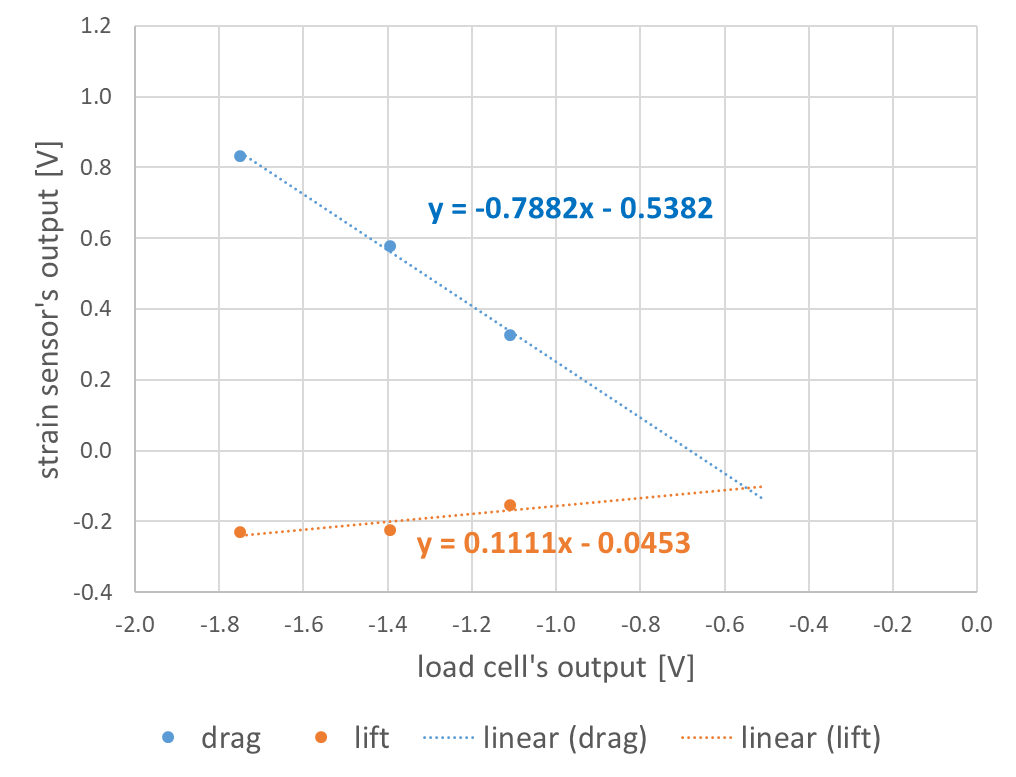
\includegraphics[width=72mm]{../images/graph_21119_drag_previous.png}
        \caption{previous data of drag}
        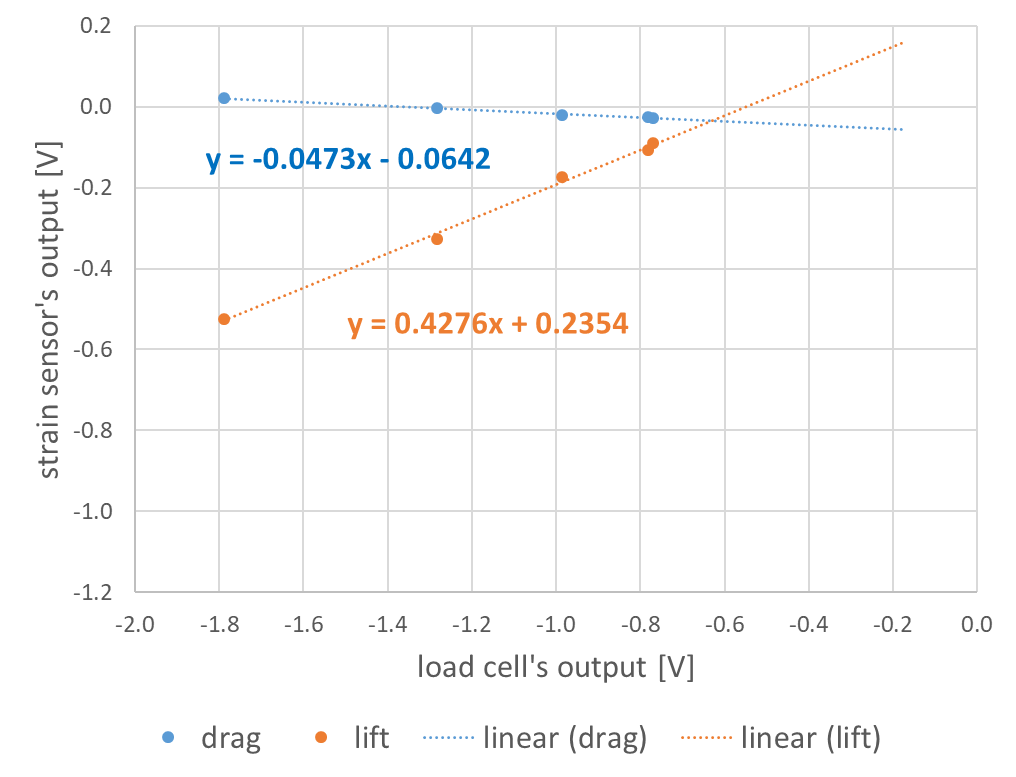
\includegraphics[width=72mm]{../images/graph_21119_lift_previous.png}
        \caption{previous data of lift}
    \end{center}
\end{figure}

\newpage
\subsection{再実施データ:抗力}
以下のFig.3~Fig.5に抗力方向の実験データを示す.
なお,ロードセルを測定ごとに再設置し実験を行った.
また,プロットしているデータは,採用点と後部の9点の計10点の平均を用いている.
\begin{figure}[htbp]
    \footnotesize
    \begin{center}
        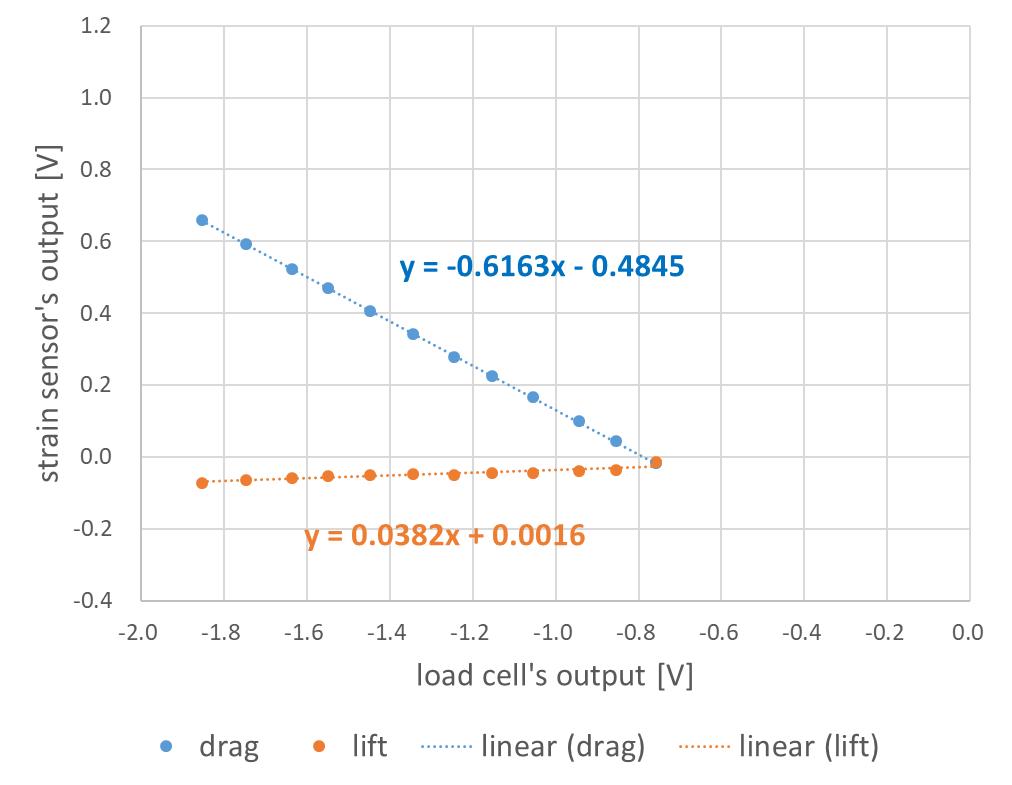
\includegraphics[width=72mm]{../images/graph_21119_drag_1.png}
        \caption{Re-experimental data of drag (1)}
        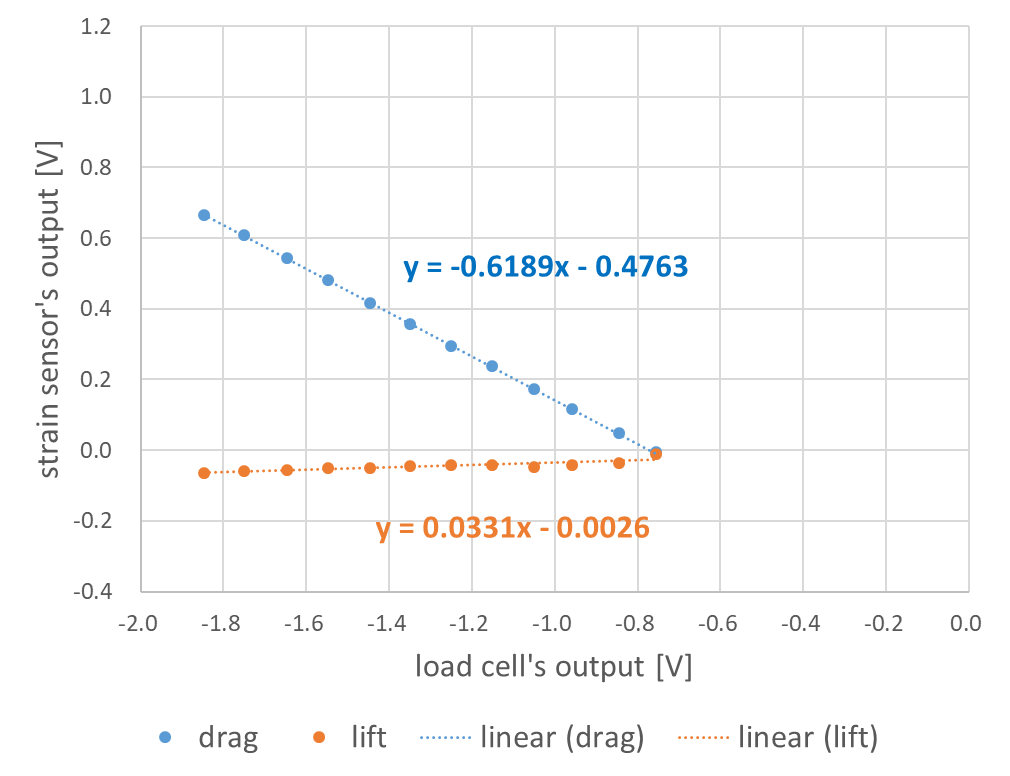
\includegraphics[width=72mm]{../images/graph_21119_drag_2.png}
        \caption{Re-experimental data of drag (2)}
        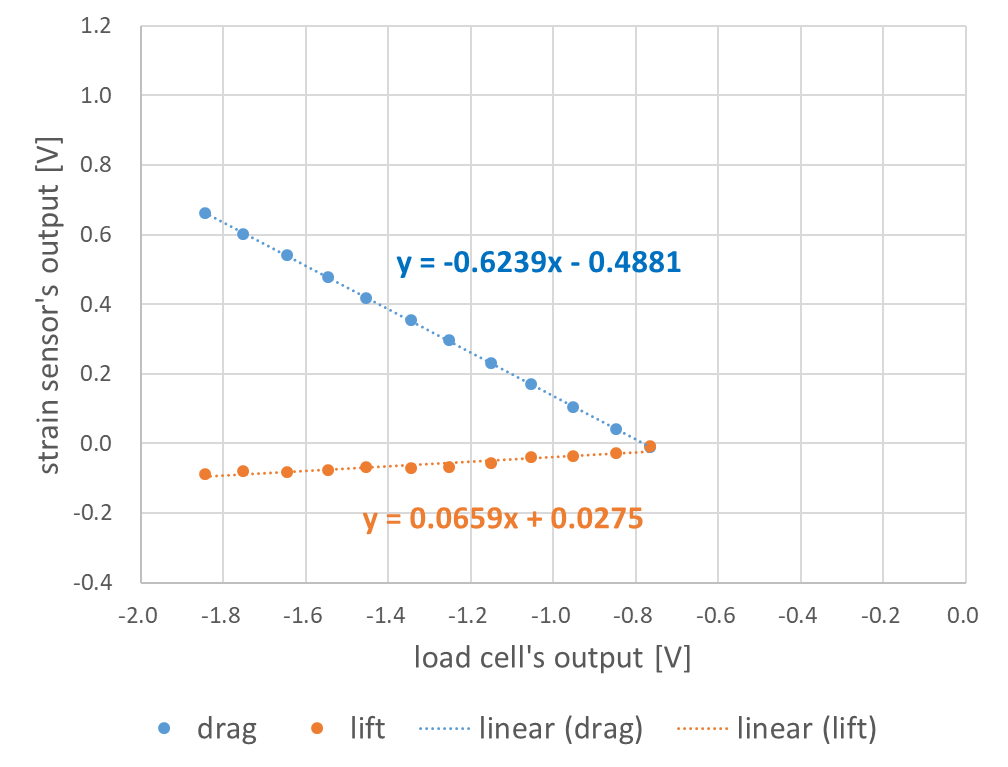
\includegraphics[width=72mm]{../images/graph_211111_drag_3.png}
        \caption{Re-experimental data of drag (3)}
    \end{center}
\end{figure}

\newpage

\subsection{再実施データ:揚力}
以下のFig.6~Fig.8に揚力方向の実験データを示す.
実験条件及びデータ解析方法は抗力方向の処理と同様である.
\begin{figure}[htbp]
    \footnotesize
    \begin{center}
        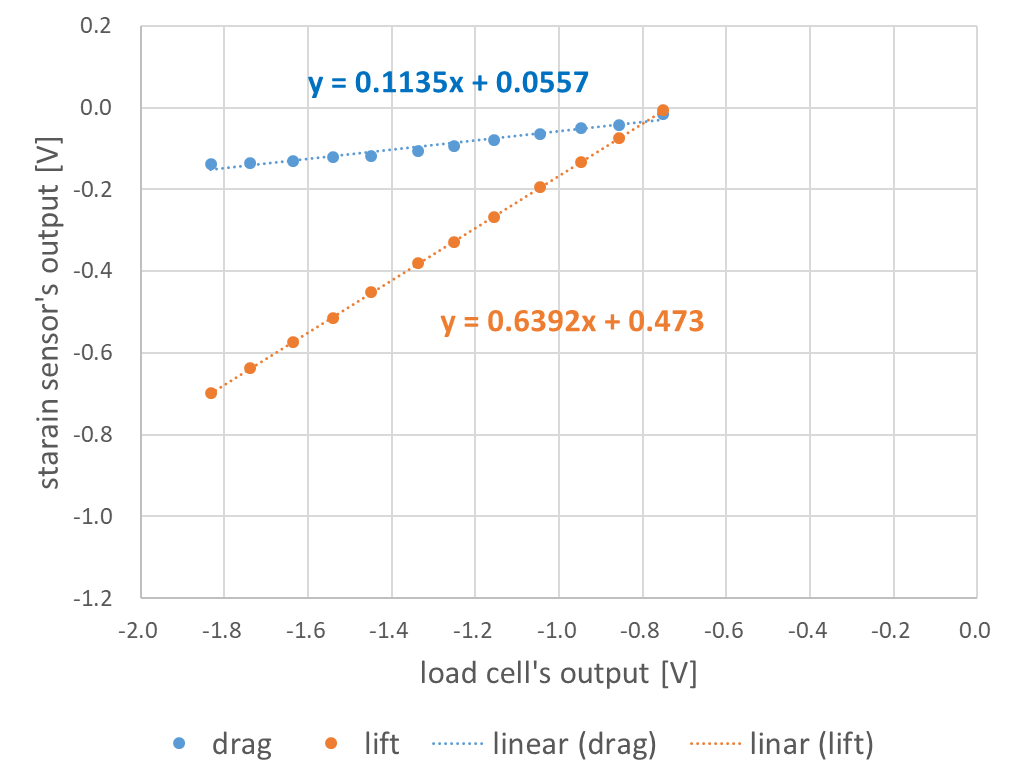
\includegraphics[width=72mm]{../images/graph_21119_lift_1.png}
        \caption{Re-experimental data of lift (1)}
        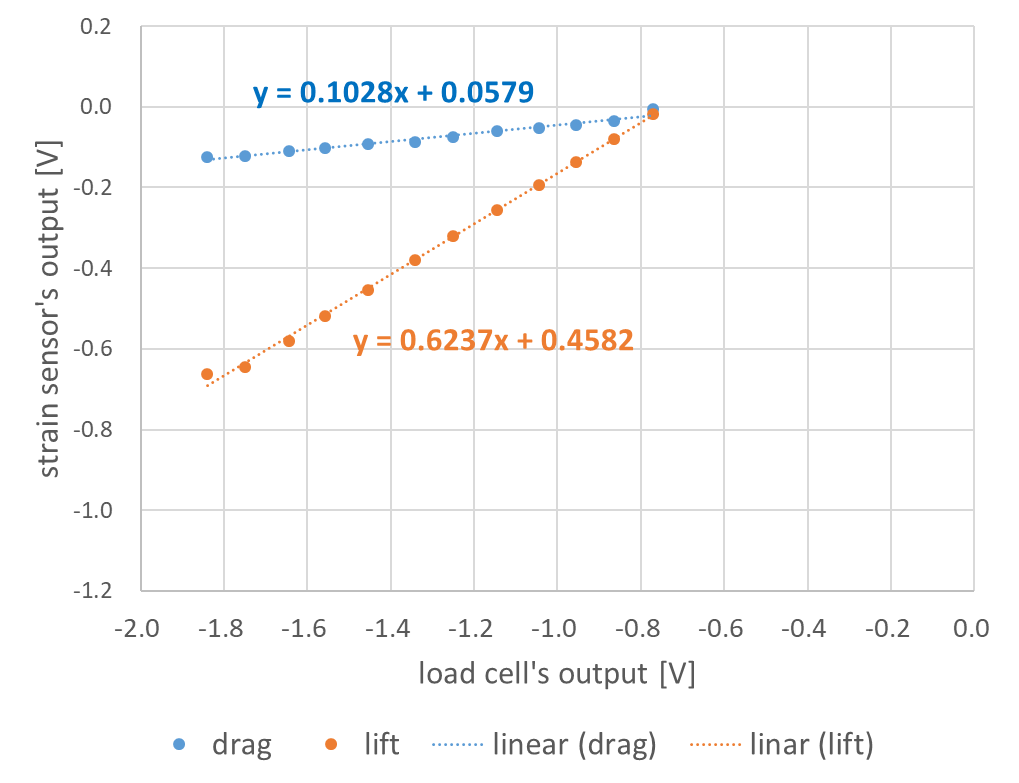
\includegraphics[width=72mm]{../images/graph_21119_lift_2.png}
        \caption{Re-experimental data of lift (2)}
        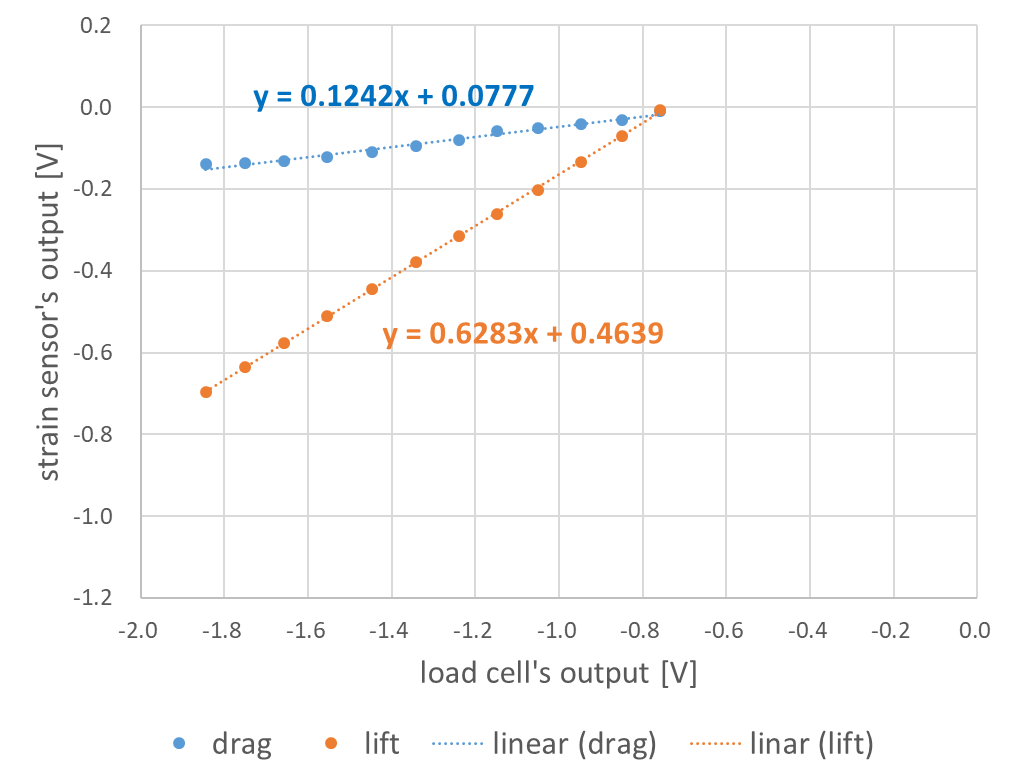
\includegraphics[width=72mm]{../images/graph_21119_lift_3.png}
        \caption{Re-experimental data of lift (3)}
    \end{center}
\end{figure}

\newpage

\section{オフセットを考慮した近似直線の算出}

\subsection{校正実験(1) ロードセルと荷重の関係}
以下のFig.9に以前行った校正実験結果を示す.
\begin{figure}[htbp]
    \footnotesize
    \begin{center}
        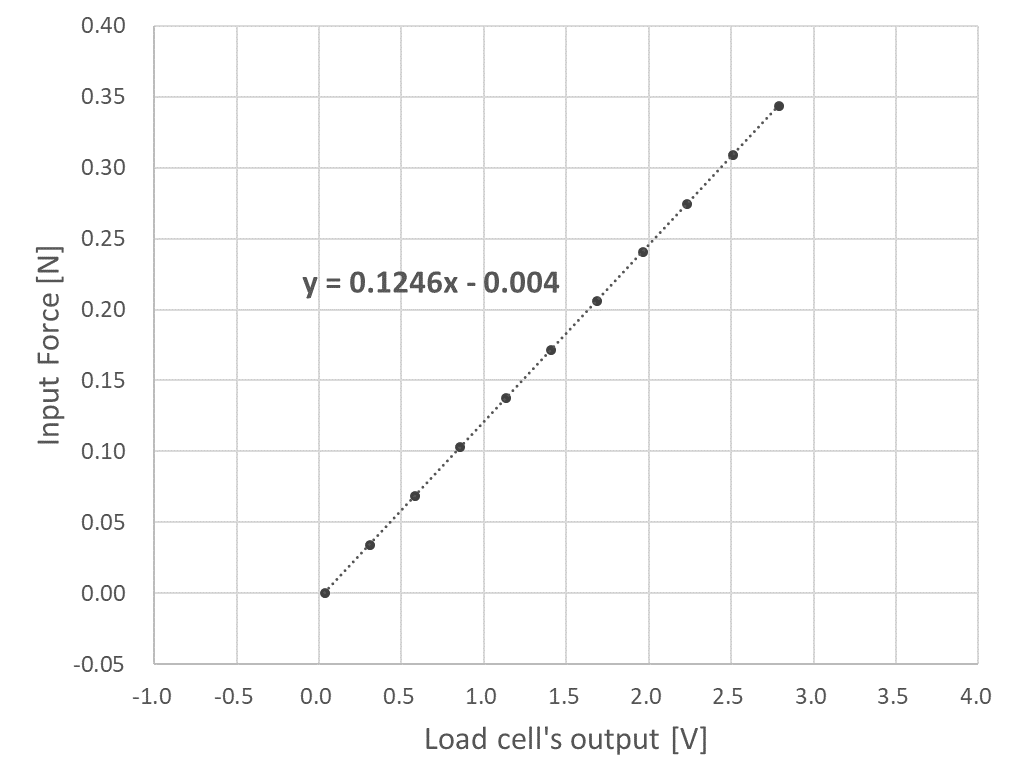
\includegraphics[width=72mm]{../images/calibration_1.png}
        \caption{Result of load cell - input force}
    \end{center}
\end{figure}

\subsection{校正実験(2) ロードセルとひずみセンサの関係}
以下のFig.10,Fig.11に以前行った校正実験結果を示す.
\begin{figure}[htbp]
    \footnotesize
    \begin{center}
        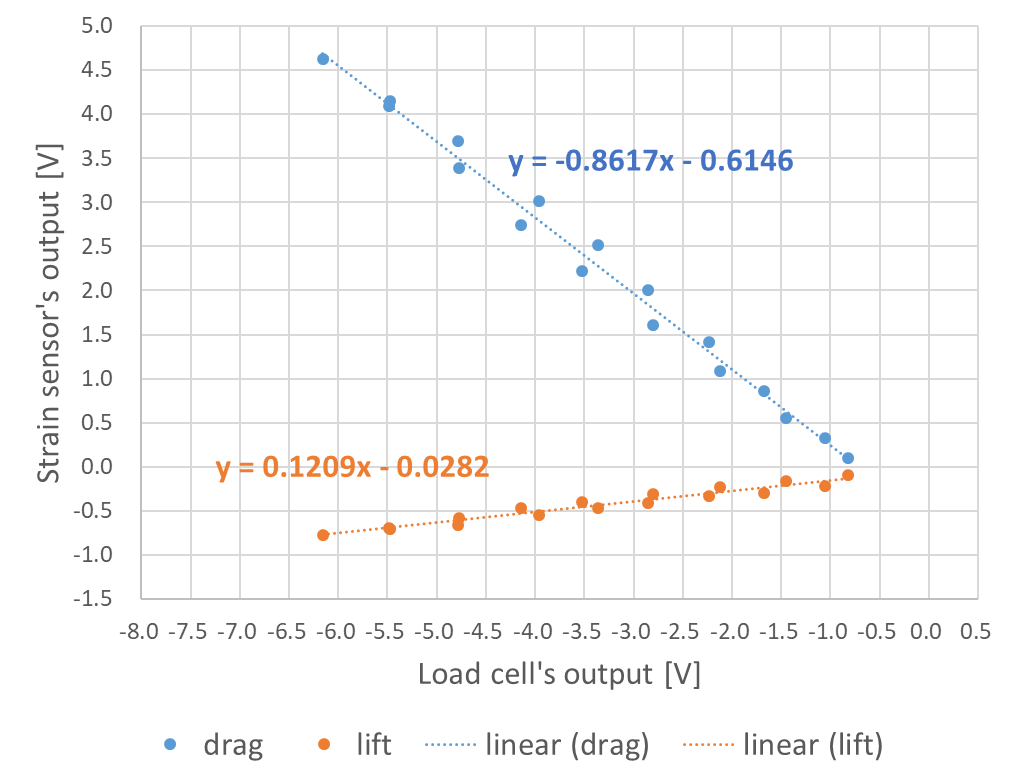
\includegraphics[width=72mm]{../images/calibration_2_drag.png}
        \caption{Result of load cell - strain sensor (drag)}
        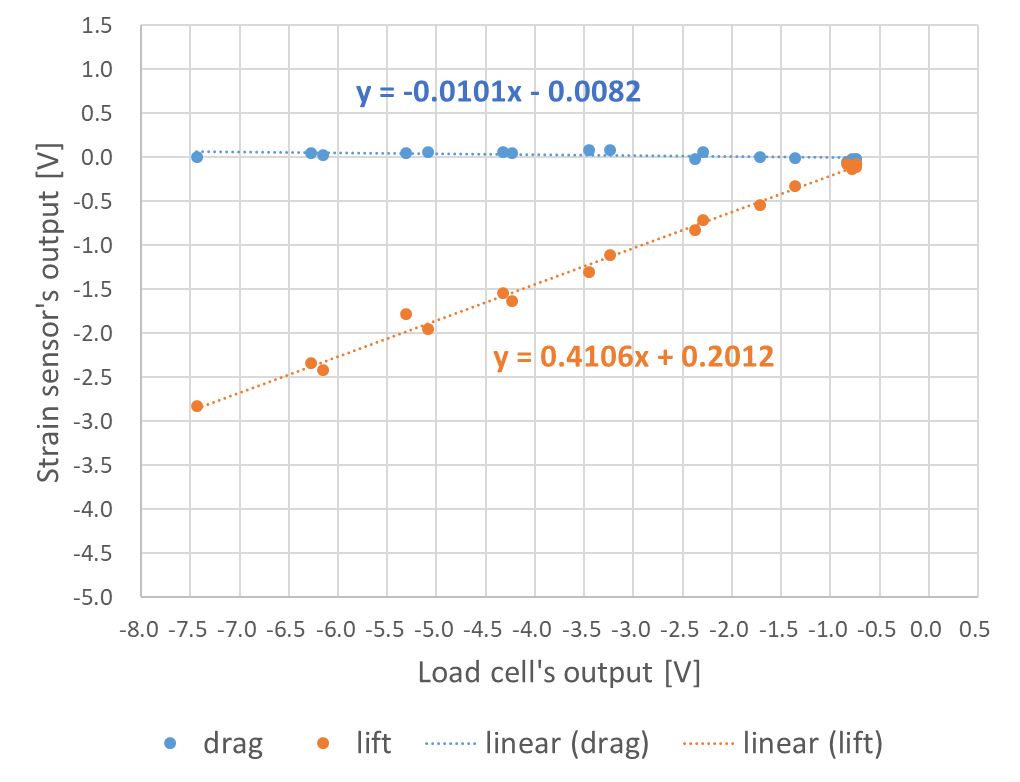
\includegraphics[width=72mm]{../images/calibration_2_lift.png}
        \caption{Result of load cell - strain sensor (lift)}
    \end{center}
\end{figure}

\newpage
\subsection{オフセット値の考慮}
実験結果から,”原点を通らない”近似直線が算出されたことから,
ロードセルのストレインアンプの出力電圧にオフセットがあると仮定した.
そのオフセット値を,実験結果のロードセルの出力電圧から差し引いた値を採用することとする.\\
\subsubsection{オフセット値の算出}
実験の際にロードセルのストレインアンプは,
バランスをとった後,0.720付近の値を示すことが多くある.
そこで,ロードセルに作用力が加えられていない状態の出力電圧を測定し,
その平均値をオフセット値として採用することとした.
算出したオフセット値は以下のようになった.
今回は,60秒間の測定値の平均を採用した.
\begin{eqnarray*}
  \mathrm{offset} = -0.728
\end{eqnarray*}

\subsubsection{オフセット値を考慮した校正実験結果}
以下のFig.12,Fig.13にストレインアンプのオフセット値を考慮した実験結果を示す.
\begin{figure}[htbp]
    \footnotesize
    \begin{center}
        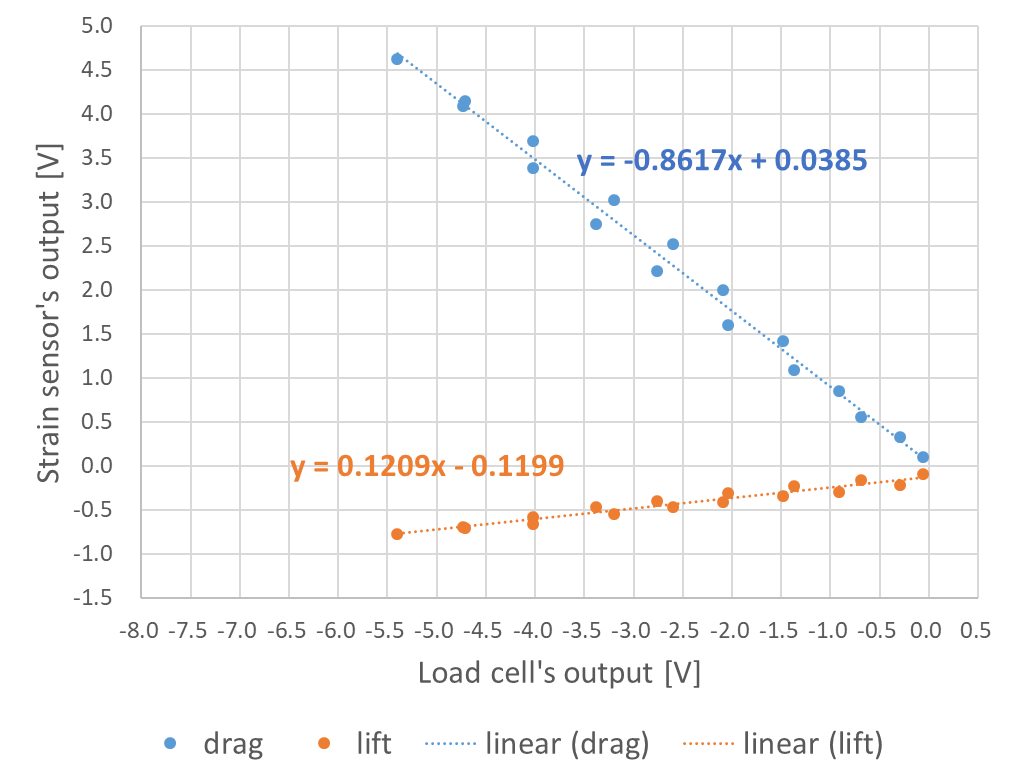
\includegraphics[width=72mm]{../images/calibration_2_drag_offset.png}
        \caption{Considered offset value (drag)}
        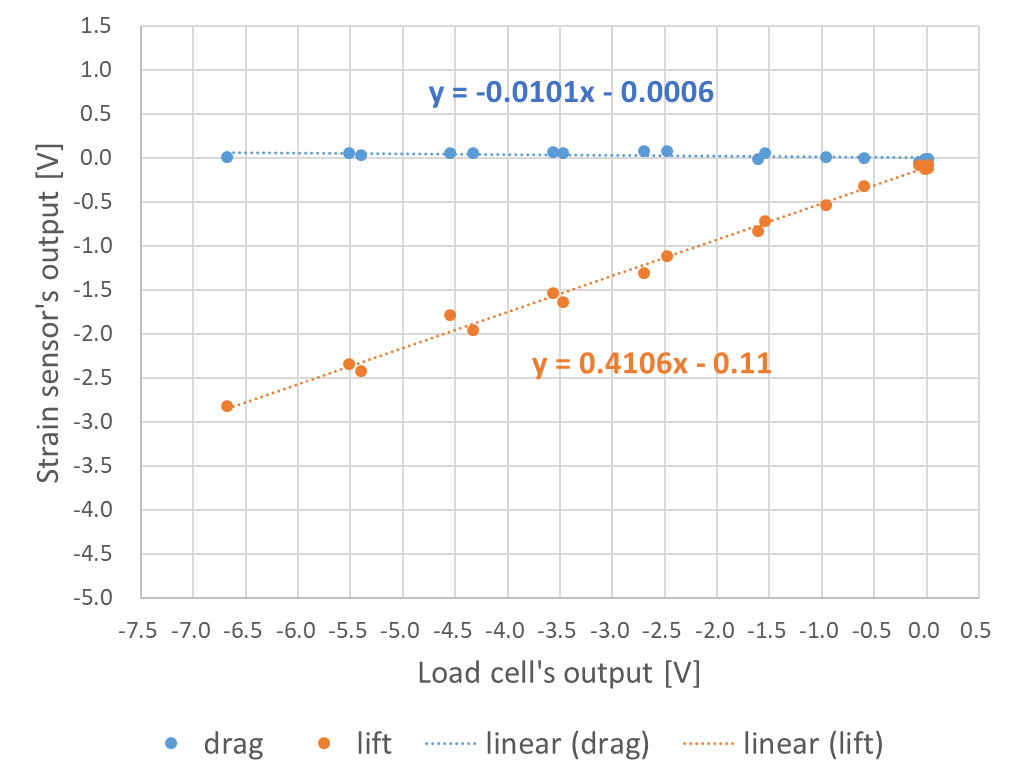
\includegraphics[width=72mm]{../images/calibration_2_lift_offset.png}
        \caption{Considered offset value (lift)}
    \end{center}
\end{figure}
\newpage

\subsection{校正実験結果を用いた換算式の算出}
同様に,入力荷重とひずみセンサの出力電圧の関係についての結果を以下のFig.14,Fig.15に示す.
なお,Fig.14はFig.10,Fig11の結果,Fig.15はFig.12,Fig13の結果を利用している.
\begin{figure}[htbp]
    \footnotesize
    \begin{center}
        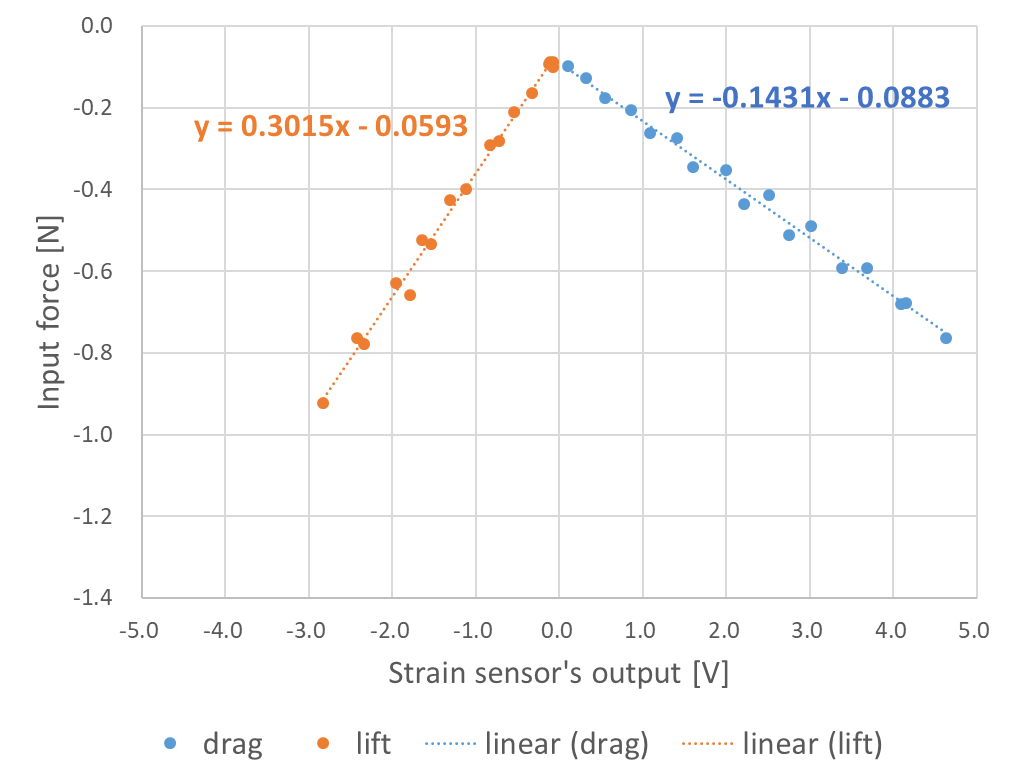
\includegraphics[width=72mm]{../images/convert.png}
        \caption{Correlation between input force and strain sensors}
        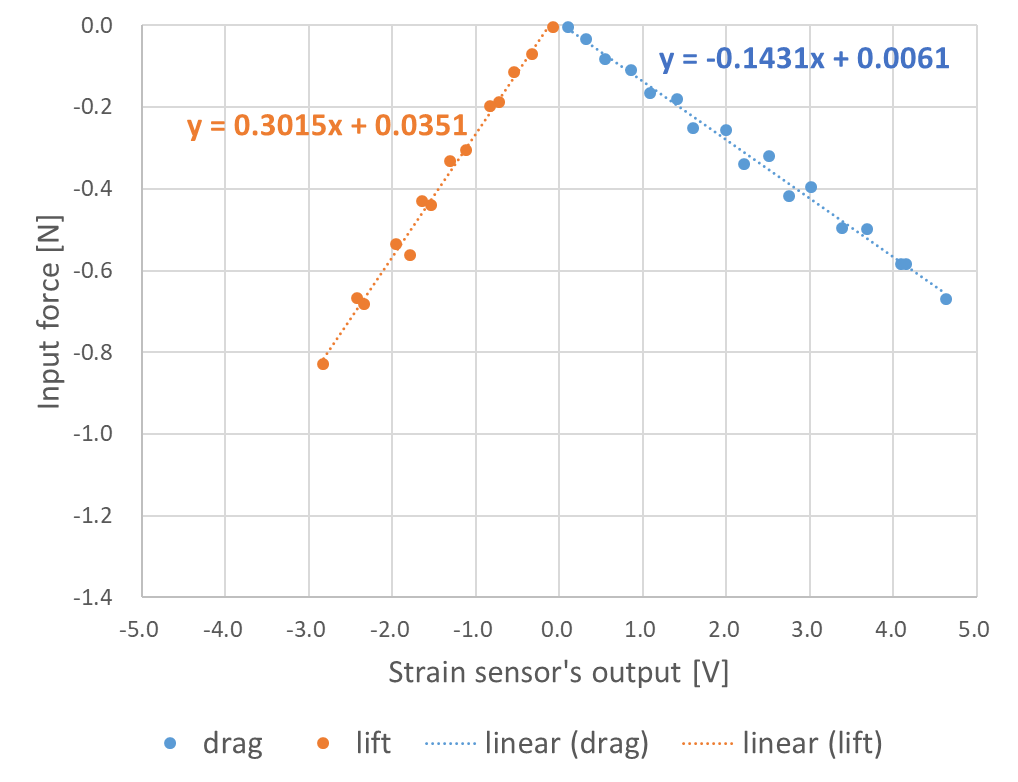
\includegraphics[width=72mm]{../images/convert_offset.png}
        \caption{Considered offset values}
    \end{center}
\end{figure}

\end{document}